\chapter{Engineering method}

% TODO: A lot of the figures/code examples look weird, need some formatting work

Intro to what will be discussed in this chapter?

% TODO: These sections below should probably be moved below the Module V.*
% sections
\section{Modularity}

Modularity is when Legos

\subsection{Granularity}

Granularity is the average? Size of the module community

\subsection{Module families}

A collection of modules that can be treated as a singular module

\subsection{Elm-Architecture}

% TODO: Insert the elm-lang architecture graph
% TODO: Also explain elm-lang

\subsection{Module Architecture}

In this application, the Elm-box is a module, while the runtime system, is the
core itself. The core invokes all modules, all of which, should have these three
functions defined:

% TODO: Add haskell code example of this

\begin{center}
  \lstinputlisting[language=Haskell,caption={Module Types}]{./code/plugin-types.hs}
\end{center}

Firstly, the types.

% TODO: Rename `Model` to `State` or something similar
\paragraph{Model}
Model is the \textit{state} of the application. In this case, it has the same
structure as a JSON object. A few values are set at the start of the
application, so it looks like this:

% TODO: Insert some code-snippet that showcases the model
% \text{\{ "location": \{ "main": \[ \] \} \}}

% TODO: Should probably explain before-hand that the core uses webview to
% display stuff.
So, the way any module inserts \gls{html} into the IDE, is by sending a tuple,
of the \gls{html}, and Location, which is where the HTML element should be
inserted. Main corresponds to the <main>-tag in a standard \gls{html} document,
like so:

html > body > main

But this introduces a possibility for some hierarchy in the module ecosystem.
For example, a module could act as a framework, and therefore needs to only be
loaded once, creating new locations, with styling.


\paragraph{*HTML}
Just a representation of \gls{html}
% TODO: Expand


\paragraph{Location}
Just a type-alias for String, to ensure type-safety
% TODO: Expand


\paragraph{Msg}
Modules create Msg-s, that are sent to all other modules that subscribe to them.

For example, if a module creates some Button, that when pressed sends
Msg "\textit{btn\-clicked}", then any module that are listening for this message,
can pick it up, when a user clicks on the button, and then optionally change the
Model.

\section{Tech Stack}

Started with Rust, because a \textit{low-level} language was assumed to be
necessary, to facilitate ease of C integration, which would allow for an
extendable application, which was language agnostic.

Framework I chose was Tauri, UI components can be created using JavaScript.

% TODO: Expand
\begin{itemize}
  \item Compiler knows when a value is unused
  \item Automatically \textit{dropped}
  \item No dangling pointers/null references
\end{itemize}

% TODO: Rewrite this to better connect to the previous section
Now just JavaScript, because nobody cares. With an \textit{agnostic} frontend,
which should be all frontends

But now the application can do this:

\begin{figure}
  \centering
  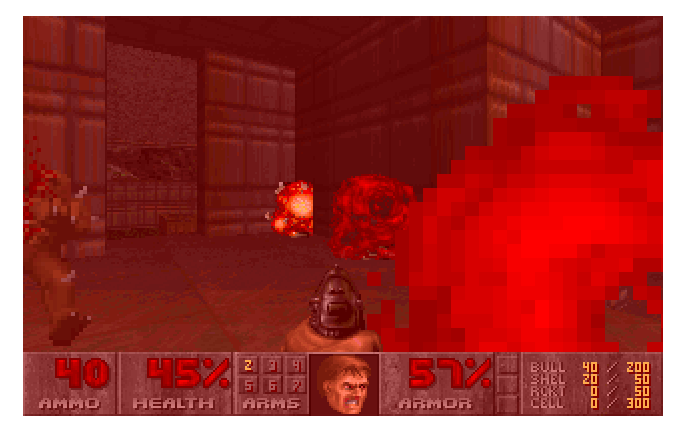
\includegraphics[scale=0.5]{./pics/doom}
  \caption{Application running Doom}
\end{figure}

% TODO: Rewrite this to better connect to the previous section
Communication between the Rust and JavaScript parts is JSON-RPC, which,
effectively, is the same as a client-server

This tech stack splits the application into two, loosely coupled parts.
\begin{itemize}
  \item Frontend (JavaScript)
  \item Backend (Rust)
\end{itemize}

Allows for modules in two different languages, with little effort. One that
targets the JavaScript environment, and one that targets Rust, with the
possibility to create bindings from Rust to C, enabling a whole sleuth of other
languages to be used.


% TODO: These sections above should probably be moved below the Module V.*
% sections

\subsection{Module V.1}

% TODO: Rewrite
First attempt was to create a Visual Studio Code Copy. This would've worked, but
would've created a lot of extra work.
Generally, the first plan was this:
\begin{enumerate}
  \item Create an IDE
  \item Extend the IDE, to allow for a module architecture
  \item Modules call the application using some DSL
\end{enumerate}

This was the \textit{easier} way to work, because I could model it of existing
% TODO: Add references here
IDEs like \textit{Visual Studio Code}. Another advantage is that when
implementing the application, I got a better understand of how eventual modules
should extend the application, like, the general architecture. But this was not
% TODO: Mention how modularity was not a concern when creating the application
modular. Anything created this way, would be subpar to existing software.

\subsection{Module V.2}

% TODO: Mention JS-MS and RS-MS

After 7–8 months of working on this, everything was scrapped for this new plan:
\begin{enumerate}
    % TODO: Add footnote
  \item Everything* is a module
\end{enumerate}

Inspired by Elm and MVC, the new module architecture would work like this:

\subsection{Architecture}
\begin{figure}
  \centering
  \begin{minted}{haskell}
-- Manifest :: Map
init :: Map
init :: [("counter", ValInt 0)]

update :: Msg -> Map -> Map
update (PluginMsg "counter") model =
  case lookup "counter" model of
    Just (ValInt i) -> insert "counter" (ValInt (i + 1)) model
    Nothing -> insert "counter" (ValInt 0) model

view :: Map -> Html
view model = Div [] [Text "Hello, World!"
  , Btn [OnClick (PluginMsg "counter")] []
  , Text (putStrLn (lookupOrDefault "counter" model))
\end{minted}



\end{figure}

To achieve this, a module would expose three methods, to be invoked by the core
application.

\paragraph{Init} Returns a collection of key-value-pairs, which represent
the state of the core.

\paragraph{Update} Returns a collection of key-value-pairs, which
overwrite existing key-value-pairs in the state, or are appended to the state.
Invoked every time a \textit{Msg} is sent.

\paragraph{View} Returns a collection which represents \gls{html},
which is rendered by the core.

This enables \textit{pureness}, if a module is pure, the whole application is
easier to reason about.

With this setup, however, the state is appending/overwriting -only, which means
the state can only grow.

This setup is also not really modular, as a single module cannot invoke another
module, without being impure. The only way to invoke/trigger another module, is
to throw a \textit{Msg}, which would trigger an update -> view - cycle. So
a module cannot \textit{listen} for a single message, all modules are triggered
by the same \textit{Msg}, and handled accordingly.

\begin{center}
  \lstinputlisting[language=Haskell, caption={Module State Types}, label=Listing]{./code/plugin-types-state.hs}
\end{center}

\begin{center}
  \centering
  \lstinputlisting[language=Haskell, caption={Module Types: Msg, HTML and Attributes State Types}, label=Listing]{./code/plugin-types.hs}
\end{center}

\begin{center}
 \lstinputlisting[language=Haskell, caption={Module Architecture}, label=Listing]{./code/plugin-architecture.hs}
\end{center}

\subsection{State Collision}

A state collision occurs when two or more modules updates the same field, during
% NOTE: Because backend-state and frontend-state was a thing
the same update-cycle. This issue also occurs when folding two states.

Was \textit{solved} with this:

\begin{minted}{haskell}
  -- TODO: The types here are wrong
  stateUpdateHandler :: State -> State -> State
  stateUpdateHandler fs bs = map foldPartition (group (fs ++ bs))

  foldPartition :: (State, [(String, State)]) -> ([String, State]) -> (State, [(String, [State])])
  foldPartition acc cur = (map snd (head cur) : fst acc, tail cur : snd acc)
\end{minted}

Takes list of states from all modules, checks for collisions. It returns a
list of `Either [(String, State)] ([(String, State)], String)`. If it is a
collision, then it's a `Right ([(String, State)], String)`, which is a tuple
where the first element is a list of tuples, being the module and their
state, and the last element being the field that the collision occurred on.
The other value: `Left [(String, State)]`, are the module state that has no
collision.

\paragraph{Collision} A collision between two states occurs if they share the same
field.

Example of the code in Haskell

\begin{center}
  \lstinputlisting[language=Haskell, caption={State Collision}, label=Listing]{./code/state-collision.hs}
\end{center}

There are several different ways to correct a collision between two
states:

\begin{enumerate}
  \item If the states are of same type:
    \begin{enumerate}
      \item If the value from one of the colliders are unchanged from the previous state:
        \begin{enumerate}
          \item Keep the new value OR Keep the old value
        \end{enumerate}
      \item Else
        \begin{enumerate}
          \item Apply the types' semigroup operator to the fields.
        \end{enumerate}
    \end{enumerate}
  \item Else
    \begin{enumerate}
      \item If the value from one of the colliders are unchanged from the previous state:
        \begin{enumerate}
          \item Keep the new value OR Keep the old value
        \end{enumerate}
      \item Else
        \begin{enumerate}
          \item Keep the left-hand side value OR Keep the right-hand side value
        \end{enumerate}
    \end{enumerate}
\end{enumerate}

Since the states are ordered by the name of the module they come from, we
have a consistent ordering of left-hand side and right-hand side, so if the same
modules give a collision on the same input, given that all modules are pure, the
resulting state will be the same every time. The problem is that applying some
function on the values could be an unwanted way to resolve collisions. So the
standard way, will be to log the collision, and then drop both states. So even
if two states have A and B amount of fields, and just one collision, we will
drop A + B amount of fields. Therefore, for a module developer, they should avoid
collisions.

% TODO: Mention how updating two fields on the same object also counts as a
% collision

This problem of resolving state collision only occurs due because each module
returns a subtree of the state. We then have to analyze the new coalesced tree
for each new subtree that is added, to figure out if there occurs any collision.
And then notifying the module developer of which field this collision occurred
on, and which modules tried to modify that field.

\subsection{Module V.3}

Third, and hopefully the final plan:

\begin{enumerate}
    % TODO: Add footnote
  \item Everything* is a module
  \item Modules can \textit{invoke} modules
\end{enumerate}

A module only exposes a singular function:

\paragraph{Init} Returns a collection of modifications


\subsubsection{Tree Manipulation}

% TODO: Mention how state and ui manipulation is equivalent to tree manipulation

This restructure changes the way the view is render. Instead of the view being
re-rendered for each state-update, the view, or \gls{ui}-hierarchy, is only
% TODO: Mention earlier how React was used/considered due to the "smart"
% re-rendering
modified by modules. This modification is similar to the earlier state
modification, so a unified algorithm to solve this can be used. If there is an
easy way to translate a \gls{ui} modification to a state modification, and back
again. To solve this, instead of having a module return the actual
modifications, meaning, the updated core, a module returns a set of instructions
of what to do with the Core.
% TODO: Add trivial module example, or something

Using this as a module developer is quite abstract, so to facilitate development
of modules, a helper class was created, which \textit{translates} modifications
to instructions. These instructions can then be analyzed for possible
collisions. This solves the edge-case of a non-colliding modification of an
object in the state.

\begin{center}
  \lstinputlisting[language=Haskell, caption={Module Type}, label=Listing]{./code/module-example.hs}
\end{center}

\begin{center}
  \lstinputlisting[language=Haskell, caption={Module Event Type}, label=Listing]{./code/module-example-event.hs}
\end{center}

\begin{center}
  \lstinputlisting[language=Haskell, caption={Module Counter Example}, label=Listing]{./code/module-example-counter.hs}
\end{center}

\begin{center}
  \lstinputlisting[language=Haskell, caption={Module Counter Example Event Handler}, label=Listing]{./code/module-example-counter-handler.hs}
\end{center}
